\section{Fichier DICOM}

\frame
{
	\frametitle{Conventions DICOM}
	\begin{itemize}
		\item Single Frame
		\begin{itemize}
			\item Une image : stock\'ee dans un fichier.
			\item Une coupe = une image
		
			$\Rightarrow$ s\'erie de 100 coupes = 100 fichiers.
		\end{itemize}
		\item Multiframe
		\begin{itemize}
			\item Aussi appel\'e \emph{Enhanced DICOM}.
			\item Plusieurs images dans la m\^eme s\'equence.
			
			E.g. s\'equence vid\'eo d'\'echographie.
		\end{itemize}
		\item Arborescence des r\'epertoires/fichiers
		\begin{center}
			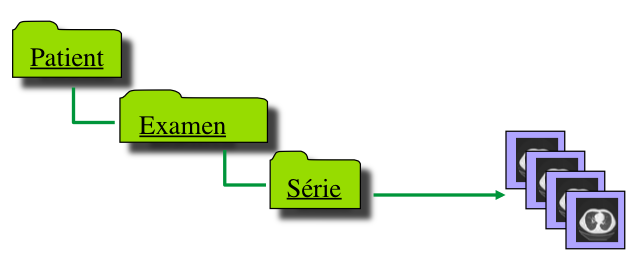
\includegraphics[width=.8\linewidth]{./figures/arborescence.png}
		\end{center}

	\end{itemize}
}

\frame
{
	\frametitle{Fichier en pratique}
	
	\begin{itemize}
		\item Peut \^etre exp\'edi\'e par messagerie.
		\item Convertible en d'autres formats (JPEG, AVI, etc.)
		\item Extension : .dcm
		\item Exemple avec OsiriX.
	\end{itemize}
}

\frame
{
	\frametitle{Contenu d'un fichier .dcm}
	
	Un fichier DICOM est l'agr\'egation des \'el\'ements suivants :
	\begin{itemize}
		\item Pr\'e-ent\^ete :
		\begin{itemize}
			\item Pr\'eambule : 128 octets de donn\'ees "application".
			\item Pr\'efixe : 0x4449434D=DICM (4 octets).
		\end{itemize}
		\item Suite de Data Elements.
		En g\'en\'eral :
		\begin{itemize}
			\item Tag ;
			\item VR ;
			\item Taille ;
			\item et Valeur.
		\end{itemize}
	\end{itemize}
}

